\section*{Ziel}
    Ziel des Versuchs ist es den Zeemann Effekt zu vermessen, wobei die Aufspaltung der Energieniveaus eines Atoms bei angelegtem äußerem Magnetfeld für das Auge sichtbar gemacht wird, um damit die Landè Faktoren für Elektronen in Cadmium zu bestimmen.

\section{Theorie}
\label{sec:theorie}

    \subsection{Grundlagen}
    \label{sec:energie} 
        Die Zustände wasserstoffähnlicher Atome mit nur einem Valenzelektron können auf den ersten Blick durch drei Quantenzahlen beschrieben werden.
        $n \in \mathbb{N}$ ist die Hauptquantenzahl, welche in die Energie des Atoms eingeht.
        $l$ ist die Drehimpulsquantenzahl, die den Betrag des Drehimpulses bestimmt:
        \begin{equation}
            \vert \vec{l} \vert = \hbar \sqrt{l \left(l + 1 \right)} \qquad \text{mit} \quad l < n
        \end{equation}
        Die magnetische Quantenzahl $m_l$ gibt die Länge des Drehimpulses entlang der z-Achse an:
        \begin{equation}
            l_z = \hbar m_l \qquad \text{mit} \quad m_l = -l, \ldots, l-1, l
        \end{equation}


    \subsection{Feinstruktur}
        Wird der Spin der Elektronen berücksichtigt, so spalten sich die berechneten Energieniveaus in feinere Niveaus auf, daher auch der Name.
        Das wird durch ein semiklassisches Modell erklärt.
        Das umlaufende Elektron wird als Kreisstrom gesehen, welcher ein magnetisches Dipolmoment erzeugt, das proportional zum Drehimpuls ist
        \begin{equation}
            \label{eqn:magnMoment}
            \vec{\mu_l} = -\frac{e}{2m_e} \vec{l} = - \frac{\mu_{\text{B}}}{\hbar} \vec{l} \;,
        \end{equation}
        wobei $\mu_{\text{B}} = \frac{e \hbar}{2 m_e}$ das Bohrsche Magneton ist.
        Nach dem Biot-Savart-Gesetz entsteht daraus ein Magnetfeld, welches mit dem magnetischen Spinmoment des Elektrons koppelt.
        \begin{equation}
            E = E_n - \vec{\mu_s} \cdot \vec{B} = E_n + \frac{\mu_0 Z e^2}{8 \pi m_e^2 r^3} \left(\vec{s} \cdot \vec{l}\right)
        \end{equation}
        Mithilfe des Gesamtdrehimpulses $\vec{j} = \vec{l} + \vec{s}$, für dessen Betrag $\vert l-s \vert \leq j \leq \vert l+s \vert$ gilt, lassen sich die Energieniveaus schreiben als
        \begin{equation}
            E = E_n + \frac{a}{2} \bigl[j(j+1) - l(l+1) - s(s+1)\bigr] \qquad \text{mit} \quad a = \frac{\mu_0 Z e^2 \hbar^2}{8 \pi m_e^2 r^3} \;.
        \end{equation}
        Durch das Einführen des Gesamtdrehimpulses wird eine andere Notation praktischer, das sogenannte Termschema:
        \begin{equation}
            \label{eqn:termschema}
            ^{2S+1}L_J
        \end{equation}
        Hierbei steht das $L$ für den Bahndrehimpuls S($l=0$), P($l=1$), D($l=2$) usw., das $S = \frac{1}{2}$ für den Spin und das $J$ für den Gesamtdrehimpuls des Elektrons.
        Der Gesamtdrehimpuls wird nach den Regeln der Drehimpulsaddition in dem Bereich von $|L - S|$ bis $|L + S|$ berechnet.
        Die Hauptquantenzahl $n$ wird nicht mehr explizit dazugeschrieben.

    \subsection{Mehrelektronen Atome}
        Jedes Elektron besitzt einen Bahndrehimpuls $\vec{l_i}$ und einen Spin $\vec{s_i}$. Diese Drehimpulse koppeln auf verschiedenste Weisen untereinander. Im Folgenden werden zwei Grenzfälle dieser Kopplungen betrachtet.

        \subsubsection*{jj-Kopplung}
            Diese Kopplung ist eine gute Näherung für schwere Atome mit einer hohen Ordnungszahl.
            Da die Feinstrukturaufspaltung proportional zu $Z^4$ ist, ist die Wechselwirkungsenergie zwischen Bahndrehimpuls und Spin desselben Elektrons bei schweren Atomen viel größer, als die Wechselwirkungsenergieen zwischen den Bahndrehimpulsen und Spins verschiedener Elektronen.
            Es koppeln also zuerst alle $\vec{l_i}$ und $\vec{s_i}$ zu $\vec{j_i} = \vec{l_i} + \vec{s_i}$ bevor die Gesamtdrehimpulse der einzelnen Elektronen zu dem Gesamtdrehimpuls
            \begin{equation}
                \vec{J} = \sum_i \vec{j_i}
            \end{equation}
            koppeln.

        \subsubsection*{LS-Kopplung}
            Diese Kopplung ist eine gute Näherung für leichte Atome mit einer niedrigen Ordnungszahl.
            Die einzelnen Bahndrehimpulse und Spins setzen sich jeweils zu einem Gesamtbahndrehimpuls
            \begin{equation}
                \vec{L} = \sum_i \vec{l_i}
            \end{equation}
            und einem Gesamtspin
            \begin{equation}
                \vec{S} = \sum_i \vec{s_i}
            \end{equation}
            zusammen.
            Diese Drehimpulse verhalten sich analog zu denen eines einzelnen Elektrons in der Abwesenheit starker Magnetfelder.
            Die beiden Drehimpulse addieren sich zu einem Gesamtdrehimpuls $\vec{J} = \vec{L} + \vec{S}$, welcher genauso behandelt werden kann wie $\vec{j}$ in wasserstoffähnlichen Atomen.
            Das heißt auch, dass das Termschema aus \autoref{eqn:termschema} verwendet werden kann, wenn für die Drehimpulse des einzelnen Elektrons die kollektiven Gesamtdrehimpulsen eingesetzt werden.

            In diesem Versuch wird diese Art der Kopplung verwendet, da sie gut zum beobachteten Spektrum der Cadmium Atome passt.

    \subsection{Energieaufspaltung im äußeren Magnetfeld}
        Bei einem angelegten Magnetfeld $\vec{B}$ werden die Energieniveaus noch weiter aufgespalten, indem die Entartung in der magnetischen Quantenzahl $m$ aufgehoben wird.
        \subsubsection*{Normaler Zeemann Effekt}
        \label{sec:normalerZeemann}
            Dieser Effekt tritt auf wenn der Spin vernachlässigt wird bzw. wenn $S=0$ also $\vec{J} = \vec{L}$ gilt.
            Es bleibt also nur noch der Gesamtbahndrehimpuls übrig, der an das äußere Magnetfeld koppelt.
            Die Wechselwirkungsenergie ist dann gegeben als
            \begin{align}
                E_{\text{ZM,}L} &= - \vec{\mu_L} \cdot \vec{B} \nonumber \\
                                &= \mu_{\text{B}} m_L B \;.
            \end{align}
            Dabei spaltet sich ein Energieniveau mit $L$ in $(2L+1)$ äquidistante Energieniveaus auf, da $m_L$ von $-L$ bis $L$ geht.

        \subsubsection*{Anomaler Zeemann Effekt}
        \label{sec:anomalerZeemann}
            Wird der Spin berücksichtigt bzw. ist $S \neq 0$, so ist die Wechselwirkungsenergie mit dem Magnetfeld gegeben als,
            \begin{equation}
                E_{\text{ZM,}J} = g_J \mu_{\text{B}} m_J B
                \label{eqn:zeeman_energy}
            \end{equation}
            wobei $\mu_B$ das Bohrsche Magneton ist und $g_J$ der Landeé-Faktor mit
            \begin{equation}
                g_J = \frac{3J(J+1) + S(S+1) - L(L+1)}{2J(J+1)}
                \label{eqn:g_J}
            \end{equation}
            ist.
            
            Der Landeé-Faktor kommt daher, dass bei der Bildung des magnetischen Moments des Spins der anomale Spin-g-Faktor $g_S = 2$ dazukommt.
            Das gesamte magnetische Moment des Gesamtdrehimpulses $\vec{J}$ ist:
            \begin{equation}
                \vec{\mu}_J = \vec{\mu}_L + \vec{\mu}_S = \frac{e \hbar}{2m_{\text{e}}} \left(g_L \vec{L} + g_S \vec{S}\right)
            \end{equation}
            $e$ ist dabei die Ladung und $m_\text{e}$ die Masse des Elektrons. $g_L = 1$ wird einfach nur zur Symmetrie dazugeschrieben.
            Da $g_L \neq g_S$ sind $\vec{J}$ und $\vec{\mu_J}$ nicht parallel und weil sich die senkrechte Komponente über die Zeit herausmittelt, wird die parallele Komponente $\mu_{\text{eff}}$ benutzt, um $g_J$ herzuleiten:
            \begin{equation}
                \mu_{\text{eff}} = \frac{(\vec{\mu} \cdot \vec{J})}{\vec{J}^2} \vec{J} = g_J \frac{q \hbar}{2m_{\text{e}}} \vec{J}
            \end{equation}
            Nach $g_J$ umgeformt ergibt sich \eqref{eqn:g_J}.


    \subsection{Auswahlregeln}
    \label{sec:auswahlregeln}
        Ist die Entartung der Energieniveaus in $m$ aufgrund eines äußeren Magnetfeldes aufgehoben, so sind nur energetische Übergänge möglich, die bestimmte Auswahlregeln befolgen.
        Die Anregung eines Atoms kann also nur passieren, wenn das absorbierte Licht die Auswahlregeln erfüllt.

        Nach einer Anregung relaxieren die Elektronen nach einer zufälligen Zeit wieder in ihren Grundzustand.
        Die dabei freiwerdende Strahlung wird gleichmäßig in alle Raumwinkel abgegeben.
        Dieser Prozess wird spontane Emission genannt und auch hierbei muss das emittierte Licht die Auswahlregeln erfülllen.

        Im folgenden bedeutet das $\Delta = $ (Endzustand) - (Anfangszustand) für die Emission von Licht:
        \begin{itemize}
            \item $\Delta J = \pm 1$
            \item $\Delta m_J = 0 \qquad$ linear pol. Licht / $\pi -$Licht
            \item $\Delta m_J = -1 \qquad$ rechtspol. Licht / $\sigma^- -$Licht
            \item $\Delta m_J = +1 \qquad$ linkspol. Licht / $\sigma^+ -$Licht
        \end{itemize}

        \subsubsection*{Normaler Zeemann Effekt in Cadmium}
            Wenn ein äußeres Magnetfeld angelegt ist, spalten sich die Zustände $^1\text{D}_2$ und $^1\text{P}_1$ anhand des normalen Zeemann Effektes auf.
            Der Übergang $^1\text{D}_2 \rightarrow ^1\text{P}_1$ mit der Wellenlänge $\lambda = \SI{643,8}{nm}$ muss deshalb die obengenannten Auswahlregeln erfüllen.
            \begin{figure}[h]
                \center
                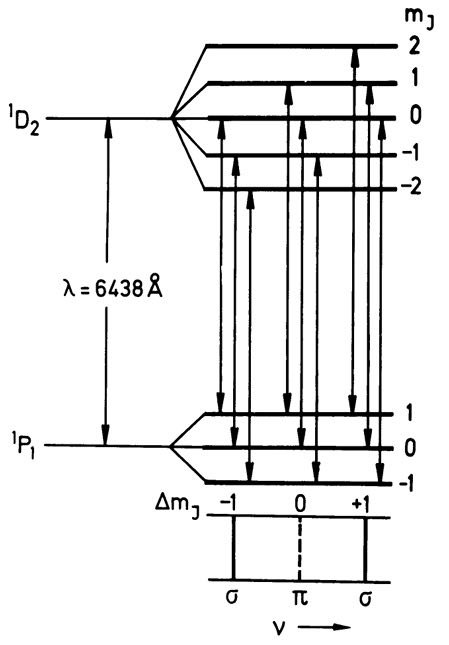
\includegraphics[width=0.35\textwidth]{bilder/normalerZeemann.jpeg}
                \caption{Die Aufspaltung der Zustände $^1\text{D}_2$ und $^1\text{P}_1$ und die möglichen Übergänge zwischen diesen Zuständen sind hier dargestellt. \cite{tu_dortmund_versuchsanleitung_2021}}
                \label{fig:normalerZeemann}
            \end{figure}
            \FloatBarrier
            
            \subsubsection*{Anomaler Zeemann Effekt in Cadmium}
            Wenn ein äußeres Magnetfeld angelegt ist, spalten sich die Zustände $^3\text{P}_2$ und $^3\text{S}_1$ anhand des anomalen Zeemann Effektes auf.
            Der Übergang $^3\text{P}_1 \rightarrow ^3\text{S}_1$ mit der Wellenlänge $\lambda = \SI{480}{nm}$ muss deshalb die obengenannten Auswahlregeln erfüllen.
            \begin{figure}[h]
                \center
                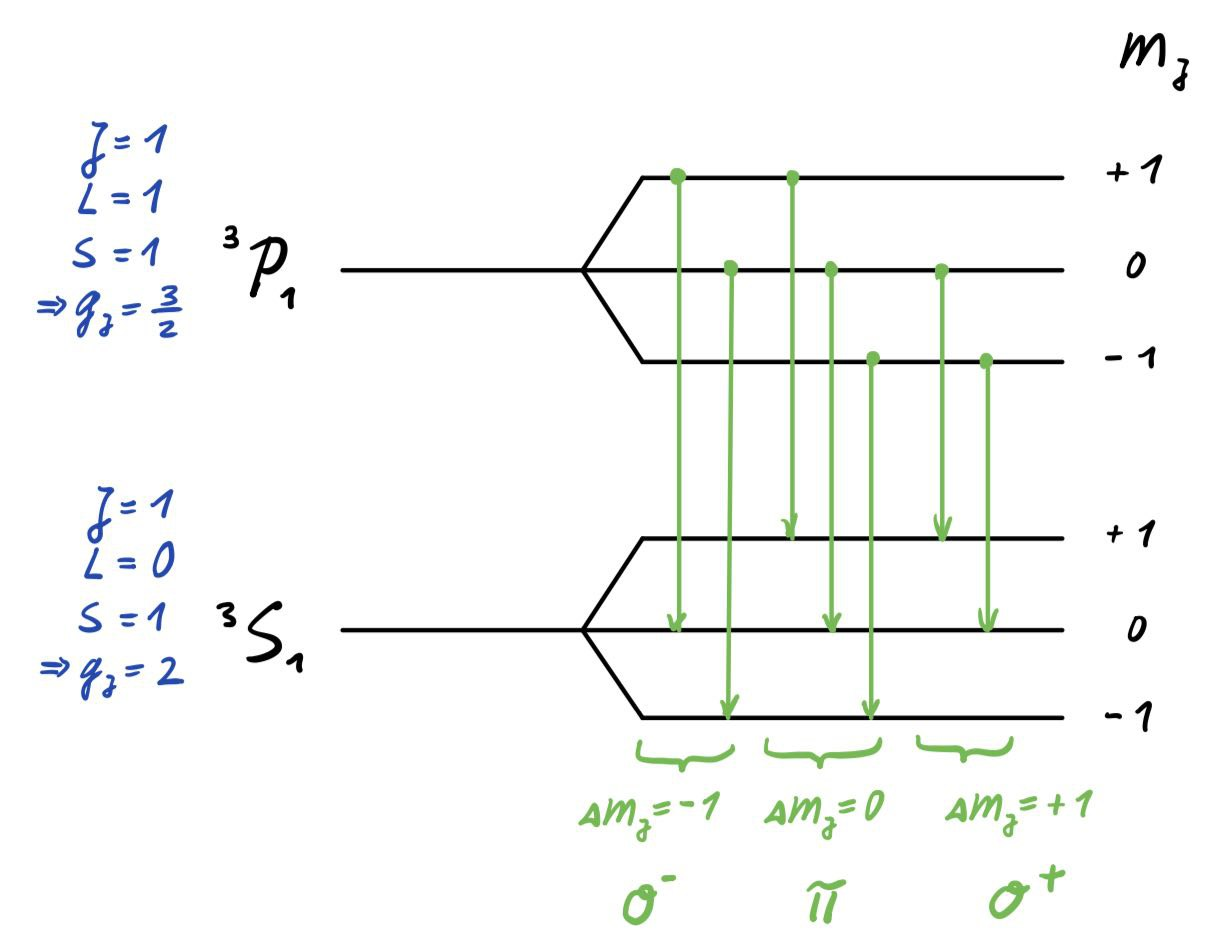
\includegraphics[width=0.7\textwidth]{bilder/anomalerZeemann.jpeg}
                \caption{Die Aufspaltung der Zustände $^1\text{D}_2$ und $^1\text{P}_1$ und die möglichen Übergänge zwischen diesen Zuständen sind hier dargestellt. \cite{tu_dortmund_versuchsanleitung_2021}}
                \label{fig:anomalerZeemann}
            \end{figure}
            \FloatBarrier
            Die Energiedifferenz zwischen zwei aufgespaltenen Energieniveaus lässt sich bestimmen aus
            \begin{equation}
                \Delta E = \bigl(g_{J,1} m_{J,1} - g_{J,2} m_{J,2}\bigr) \mu_{\text{B}} B \;.
            \end{equation}


    \subsection{Lummer-Gehrcke-Platte}
    \label{sec:platte}
        \begin{figure}[h]
            \center
            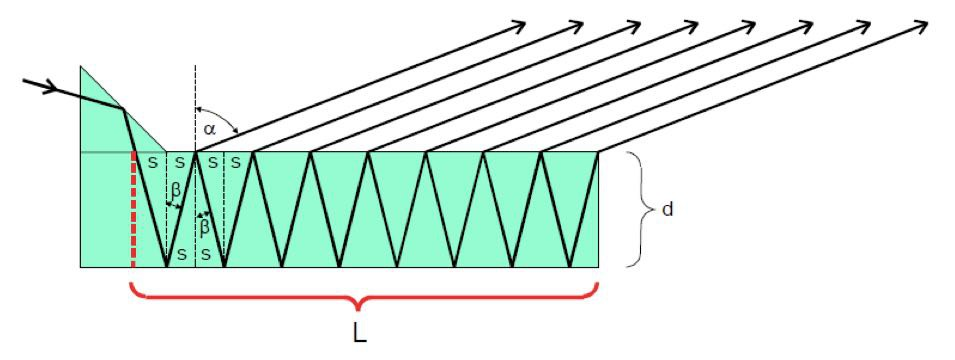
\includegraphics[width=0.7\textwidth]{bilder/LummerGehrckePlatte.jpeg}
            \caption{Die Funktionsweise der Lummer Gehrcke Platte ist hier schematisch aufgezeigt. \cite{tu_dortmund_versuchsanleitung_2021}}
            \label{fig:LummerGehrckePlatte}
        \end{figure}
        \FloatBarrier

        Licht tritt durch ein Eingangfenster ein und wird innerhalb der Platte an den Grenzflächen reflektiert und transmittiert.
        Bei jeder Reflektion tritt ein Anteil aus der Platte aus.
        Diese transmittierten Anteile interferieren miteinander, wobei die Bragg-Bedingung
        \begin{equation}
            2 n d \cos(\beta) = m \lambda \qquad \text{mit} \quad m \in \mathbb{N} \;,
        \end{equation}
        erfüllt sein muss, um konstruktive Interferenz zu erhalten.
        Dabei ist $n$ der Brechungsindex, $d$ die Dicke der Platte, $\beta$ der Reflexionswinkel und $m$ die Ordnung des Interferenzmaximas.
        \\
        Wird das Magnetfeld eingeschaltet so verändert sich die Wellenlänge des eingestrahlten Lichtes um
        \begin{equation}
            \delta \lambda = \frac{1}{2} \frac{\delta s}{\Delta s} \Delta \lambda_D \;,
        \end{equation}
        wobei $\Delta s$ der Abstand der Interferenzmaxima bei ausgeschaltetem Magnetfeld ist und $\delta s$ der Abstand der aufgespaltenen Linien bei angeschaltetem Magnetfeld ist.

        Das Dispersionsgebiet
        \begin{equation}
            \Delta \lambda_D = \frac{\lambda^2}{2 d} \sqrt{\frac{1}{n^2 - 1}}
        \end{equation}
        gibt die maximale Wellenlängendifferenz zweier aufgespaltener Wellenlängen an, sodass sich die unterschiedlichen Ordnungen der Interferenzmaxima nicht überlagern.
        Das Auflösungsvermögen $A$ einer bestimmten Wellenlänge ist gegeben als
        \begin{equation}
            A = \frac{L}{\lambda} (n^2 - 1) \;,
        \end{equation}
        wobei $L$ die Länge der Platte ist.
        
        Mit den gegebenen Werten ergeben sich die Dispersionsgebiete und Auflösevermögen für den Übergang mit \SI{643,8}{nm} als
        \begin{align*}
            \Delta \lambda_D = \SI{48,91}{pm} \\
            A = 2,09 \cdot 10^5
        \end{align*}
        und für den Übergang mit \SI{480}{nm} als
        \begin{align*}
            \Delta \lambda_D = \SI{26,95}{pm} \\
            A = 2,85 \cdot 10^5 \;.
        \end{align*}
